\documentclass{report}

\usepackage[utf8]{inputenc}

\usepackage[margin=0.75in]{geometry}
\usepackage[titletoc,title]{appendix}

% Odkomentuj by zmienić tytuł abstraktu
% \renewcommand{\abstractname}{Podsumowanie}

% Wcięcie pierwszego paragrafu po rozpoczęciu sekcji, inaczej wygląda dziwnie tbh
\usepackage{indentfirst}

% Matematyka
% https://www.overleaf.com/learn/latex/Mathematical_expressions
% https://en.wikibooks.org/wiki/LaTeX/Mathematics
\usepackage{amsmath,amsfonts,amssymb,mathtools,amsthm,empheq,mathabx}

\usepackage{polski}
\numberwithin{equation}{section}

\usepackage[figurename=Fig.]{caption}
\usepackage{fancyhdr}
\usepackage{enumitem}
\usepackage[ocgcolorlinks]{hyperref}
\hypersetup{
    ocgcolorlinks=true,
    linkcolor=blue!50!red,
    urlcolor=blue!70!black
}

% Obrazki i wykresy
% https://www.overleaf.com/learn/latex/Inserting_Images
% https://en.wikibooks.org/wiki/LaTeX/Floats,_Figures_and_Captions
\usepackage{tikz}
\usepackage{graphicx,float,pgfplots,float}
\pgfplotsset{compat=newest}
\usetikzlibrary{decorations.markings}
\graphicspath{ {./images/} }
% Algorytmy
% https://www.overleaf.com/learn/latex/algorithms
% https://en.wikibooks.org/wiki/LaTeX/Algorithms
\usepackage[ruled,vlined]{algorithm2e}
\usepackage{algorithmic}

% Wyświetlanie SVG, wymaga Inkscape'a
% \usepackage{svg}
% Syntax highlighting
% https://www.overleaf.com/learn/latex/Code_Highlighting_with_minted
\usepackage{minted}
\usemintedstyle{borland}
\renewcommand{\chaptername}{Zadanie}
\def\chapterautorefname{Zadaniu}

\title{WCYB Projekt 2}
\author{Jakub Bliźniuk}
\date{January 2023}


\begin{document}
\pagestyle{fancy}
\fancyfoot{}
\fancyfoot[C]{\thepage}
\fancyfoot[R]{324904}

\begin{titlepage}
    \vfill
    \maketitle
    \thispagestyle{fancy}
\end{titlepage}
\tableofcontents
\thispagestyle{fancy}
\setcounter{chapter}{4}
\chapter{Serwer zdalny VPN}
\label{chap:vpn}
\section{Wybrana technologia VPN}
Jako preferowaną technologię wybrałem \href{https://tailscale.com}{Tailscale}\footnote{Tailscale to oparta o Wireguard sieć overlay. Cały produkt składa się z SaaS w postaci serwera kontrolnego i "awaryjnej" sieci przez którą routowany jest ruch w przypadku (rzadkiego) niepowodzenia przebicia się przez NAT/firewall, oraz aplikacji klienckich. Więcej szczegółów można znaleźć pod \url{https://tailscale.com/}}, z self-hostowanym serwerem kontrolnym - \href{https://github.com/juanfont/headscale}{Headscale}\footnote{Headscale to otwartoźródłowa wersja serwera kontrolnego Tailscale utrzymywana przez społeczność i pracowników Tailscale w ich wolnym czasie. Można ją znaleźć pod \url{https://github.com/juanfont/headscale}}. Jest to w zasadzie technologia \textit{overlay networking}, pozwalająca na dynamiczne tworzenie połączeń między urządzeniami w sieci z użyciem Wireguard.

Konfiguracja była więc podzielona na trzy części:
\begin{enumerate}
    \item Konfiguracja serwera kontrolnego, który zarządza siecią, autoryzuje połączenia i uwierzytelnia węzły
    \item Konfiguracja węzła wychodzącego, w tym wypadku na tym samym urządzniu co serwer kontrolny
    \item Zalogowanie się do sieci w aplikacji Tailscale na urządzeniach końcowych
\end{enumerate}

Dodatkowo sieć została wykorzystana w kolejnym realizowanym \autoref{chap:pihole}, co wymagało tylko jednej zmiany w konfiguracji urządzeń wykorzystanych w tym zadaniu.

\section{Przygotowanie maszyny wirtualnej}
Na potrzebę tego zadania stworzona została jedna maszyna wirtualna w Oracle Cloud Infrastructure (OCI) o następującej specyfikacji:
\begin{itemize}
    \item 1 rdzeń ARM Ampere Altra
    \item 6 GB RAM
    \item 1 gigabitowa karta sieciowa
    \item dysk 47GB (domyślny i jednocześnie minimalny rozmiar)
    \item system Oracle Linux (bazowany na RHEL)
\end{itemize}
Wygenerowany w OCI plik Terraform z którego ta maszyna została stworzona - z usuniętymi informacjami unikalnymi do użytego konta (identyfikator OCID sieci i projektu, klucz publiczny SSH) - znajduje się w \href{https://github.com/oplik0/WCYB-Projekt-2}{repozytorium projektu}\footnote{Link do pliku w repozytorium: \url{https://github.com/oplik0/WCYB-Projekt-2/blob/main/wcyb-machine.tf}}

\section{Konfiguracja Headscale}

W celu skonfigurowania serwera kontrolnego na Linuxie wystarczy podążałem za \href{https://github.com/juanfont/headscale/blob/main/docs/running-headscale-linux.md}{instrukcjami z repozytorium Headscale}. Kolejne kroki wyglądały następująco:

\subsection{Przygotowanie plików}

\subsubsection{Pobranie Headscale}

Headscale kompiluje się do jednego pliku wykonywalnego, który wystarczy pobrać z  ich GitHuba

\begin{minted}{bash}
wget --output-document=/bin/headscale \
https://github.com/juanfont/headscale/releases/download/v0.18.0-beta2/headscale_0.18.0-beta2_linux_arm64
\end{minted}

Warto też sprawdzić sumę kontrolną z opublikowanymi, co można zrobić komendą \mintinline{bash}{sha256sum}, co w przypadku \mintinline{go}{0.18.0-beta2} powinno wyglądać tak:

\begin{minted}{bash}
$ sha256sum /bin/headscale
e5d453352bc06fb1ffd6a16f973b40311f924e52006fe3c7d4ee227535a4153f  /bin/headscale
\end{minted}

Następnie należy upewnić się, że plik jest wykonywalny

\begin{minted}{bash}
sudo chmod +x /bin/headscale
\end{minted}

\subsection{Przygotowanie użytkownika i reszty plików}

\subsubsection{Folder na konfigurację}

Następnie należy stworzyć folder który będzie wykorzystywany do konfiguracji Headscale

\begin{minted}{bash}
sudo mkdir -p /etc/headscale
\end{minted}

\subsubsection{Stworzenie użytkownika}

W tym momencie można też już stworzyć użytkownika do usługi, co pozwoli nam też od razu stworzyć folder na dane zmienianie w czasie działania programu
\begin{minted}{bash}
sudo useradd \
	--create-home \
	--home-dir /var/lib/headscale/ \
	--system \
	--user-group \
	--shell /usr/bin/nologin \
	headscale    
\end{minted}

\subsubsection{Stworzenie pustego pliku bazy danych}

\begin{minted}{bash}
    sudo -u headscale touch /var/lib/headscale/db.sqlite
\end{minted}

\subsubsection{Stworzenie pliku konfiguracyjnego}

Możemy w tym momencie stworzyć też pusty plik konfiguracyjny, ale prościej jest zacząć od \linebreak
\href{https://github.com/juanfont/headscale/blob/main/config-example.yaml}{przykładowej konfiguracji z repozytorium Headscale}\footnote{\url{https://github.com/juanfont/headscale/blob/main/config-example.yaml}} - najprościej to zrobić po prostu przeklejając tekst z użyciem preferowanego edytora tekstu

\begin{minted}{bash}
sudoedit /etc/headscale/config.yaml
\end{minted}

Można już też w tym momencie edytować konfigurację - ostateczna wersja z którą skończyłem (z usuniętymi identyfikatorami i sekretem OpenID Connect) znajduje się w \href{https://github.com/oplik0/WCYB-Projekt-2/blob/main/config.yaml}{Repozytorium projektu}\footnote{Link do pliku: \url{https://github.com/oplik0/WCYB-Projekt-2/blob/main/config.yaml}}

\subsubsection{Konfiguracja ACL}
Domyślnie każdy użytkownik ma dostęp tylko do swoich urządzeń. Można jednak to zmienić, a także pozwolić wykonywać połączenia poza sieć wirtualną, ustawiając listy kontroli dostępu. Wykorzystana przeze mnie konfiguracja pobiera listy z pliku \mintinline{bash}{/etc/headscale/acl.jsonc}. Kopia wykorzystanego przeze mnie pliku znajduje się w \href{https://github.com/oplik0/WCYB-Projekt-2/blob/main/acl.jsonc}{repozytorium projektu pod nazwą \mintinline{bash}{acl.jsonc}}\footnote{Link do pliku ACL: \url{https://github.com/oplik0/WCYB-Projekt-2/blob/main/acl.jsonc}}
\begin{samepage}
\subsection{Konfiguracja usługi}
W tym momencie headscale powinno już działać, co można sprawdzić komendą \mintinline{bash}{headscale serve} - lepszym pomysłem niż manualne uruchamianie jest jednak stworzenie usługi SystemD - co możemy zrobić tworząc plik \mintinline{bash}{/etc/systemd/system/headscale.service}, np. używając edytora przez \mintinline{bash}{sudoedit /etc/systemd/system/headscale.service}.
Zawartość pliku powinna wyglądać następująco:
\begin{minted}{ini}
[Unit]
Description=headscale controller
After=syslog.target
After=network.target

[Service]
Type=simple
User=headscale
Group=headscale
ExecStart=/bin/headscale serve
Restart=always
RestartSec=5

# Optional security enhancements
NoNewPrivileges=yes
PrivateTmp=yes
ProtectSystem=strict
ProtectHome=yes
ReadWritePaths=/var/lib/headscale /var/run/headscale
AmbientCapabilities=CAP_NET_BIND_SERVICE
RuntimeDirectory=headscale

[Install]
WantedBy=multi-user.target
\end{minted}
\end{samepage}

\subsection{Otwieranie portów w firewallu}
\subsubsection{Otworzenie gRPC i STUN}
Headscale wystawia usługi na kilku potrach. W konfiguracji z którą skończyłem dwie z nich powinny być wystawione do internetu - gRPC i STUN. Możemy je przepuścić na serwerze komendą \mintinline{bash}{firewall-cmd}:
\begin{minted}{bash}
sudo firewall-cmd --add-port=50443/tcp --permanent
sudo firewall-cmd --add-port=3478/tcp --permanent
sudo firewall-cmd --reload
\end{minted}
Przez wykorzystanie Oracle Cloud Infrastructure należało te porty przepuścić też na listach bezpieczeństwa w sieci wirtualnej w OCI, co jednak zrobiłem wcześniej.
\subsubsection{Otworzenie portów HTTP(S)}
Tailscale do kontroli wykorzystuje też protokół HTTP(S). Konfiguracja Tailscale nie wystawia go na zewnątrz - zmiast tego posłuży do tego serwer nginx, co pozwoli też dodać statyczną stronę do zarządzania serwerem (korzystając z projektu \href{https://github.com/gurucomputing/headscale-ui}{headscale-ui}). Ponownie robimy to z pomocą \mintinline{bash}{firewall-cmd}, tym razem jednak istnieją już predefiniowane usługi:
\begin{minted}{bash}
sudo firewall-cmd --add-service=http --permanent
sudo firewall-cmd --add-service=https --permanent
sudo firewall-cmd --reload
\end{minted}
\subsection{Uruchomienie usługi}
Ostatnim krokiem jest uruchomienie Headscale i sprawdzenie czy działa. Wystarczy do tego przeładować usługi systemd i włączyć stworzoną wcześniej usługę:
\begin{minted}{bash}
sudo systemctl daemon-reload
sudo systemctl enable --now headscale
\end{minted}
Możemy teraz sprawdzić status usługi komendą \mintinline{bash}{systemctl status headscale} i upewnić się, że wszystko działa poprwnie sprawdzając wystawione metryki z użyciem \mintinline{bash}{curl http://127.0.0.1:9090/metrics}

\section{Headscale-UI i nginx}

Jednym elementem którego brakuje w Headscale w stosunku do oferty SaaS jest panel administratora. Istnieje jednak osobny projekt adresujący tę potrzebę, nawet jeśli nie jest jeszcze na poziomie oficjalnego rozwiązania. \href{https://github.com/gurucomputing/headscale-ui}{Headscale-UI} jest prostą stroną statyczną napisaną w SvelteKit. Możemy ją serwować wykorzystując nginx jako proxy do zarówno headscale jak i panelu, wystawiając je pod tą samą domeną.

\subsection{Pobranie Headscale-UI}

W repozytorium projektu jako wydania publikowane są pliki zip zawierające zbudowaną wersję strony. Możemy więc dość łatwo pobrać projekt i go rozpakować do \mintinline{bash}{/srv}:
\begin{minted}{bash}
wget --output-document=/srv/headscale-ui.zip \
https://github.com/gurucomputing/headscale-ui/releases/download/2022.12.23.2-beta/headscale-ui.zip

unzip /srv/headscale-ui.zip
\end{minted}
Przez wykorzystanie SELinuxa w Oracle Linux należy też odpowiednio oznaczyć pliki by nginx miał do nich później dostęp:
\begin{minted}{bash}
semanage fcontext -a -t httpd_sys_content_t "/srv/headscale-ui(/.*)?"
restorecon -Rv /srv/headscale-ui
\end{minted}
\subsection{Instalacja nginx}

W przypadku Oracle Linux nginx należy zainstalować korzystając z menadżera pakietów \mintinline{bash}{dnf} (lub starszego \mintinline{bash}{yum}). Inne dystrybucje mogą używać innych menedżerów pakietów (np. \mintinline{bash}{apt} w Debianie/Ubuntu):

\begin{minted}{bash}
sudo dnf install nginx
\end{minted}

Przy okazji można też zainstalować narzędzie certbot które można wykorzystać do wygenerowania certyfikatów dla domeny na której będzie serwowana strona i headscale:

\begin{minted}{bash}
sudo dnf install certbot python3-certbot-nginx
\end{minted}

\begin{samepage}    
\subsection{Konfiguracja nginx}
Następnie należy stworzyć konfigurację nginx - to co ważne to zdefiniowane dwóch bloków \mintinline{bash}{location}:
\begin{minted}{yaml}
    location /web {
            alias /srv/headscale-ui/;
            index index.html;
    }
    location / {
        proxy_pass http://127.0.0.1:8080;
        proxy_http_version 1.1;
        proxy_set_header Upgrade $http_upgrade;
        proxy_set_header Connection $connection_upgrade;
        proxy_set_header Host $server_name;
        proxy_redirect http:// https://;
        proxy_buffering off;
        proxy_set_header X-Real-IP $remote_addr;
        proxy_set_header X-Forwarded-For $proxy_add_x_forwarded_for;
        proxy_set_header X-Forwarded-Proto $http_x_forwarded_proto;
        add_header Strict-Transport-Security "max-age=15552000; includeSubDomains" always;
    }
\end{minted}
Ostateczna konfiguracja z którą skończyłem, po dodatkowym wykorzystaniu narzędzia certbot w celu wygenerowania certyfikatów TLS dla domeny, znajduje się w \href{https://github.com/oplik0/WCYB-Projekt-2/blob/main/headscale.conf}{repozytorium projektu jako headscale.conf}\footnote{Link do pliku: \url{https://github.com/oplik0/WCYB-Projekt-2/blob/main/headscale.conf}}
\end{samepage}

\subsection{Uruchomienie nginx}

Po skonfigurowaniu wystarczy włączyć usługę:
\begin{minted}{bash}
sudo systemctl enable --now nginx
\end{minted}

\subsection{pobranie klucza API}
By móc połączyć panel administracyjny z API Headscale należy wygenerować klucz na serwerze używając komendy
\begin{minted}{bash}
headscale apikeys create
\end{minted}
Po wklejeniu go w ustawieniach panelu zostanie on zapisany lokalnie w przeglądarce (krok ten trzeba więc powtarzać na każdym urządzeniu), co pozwoli nam zarządzać użytkownikami i urządzeniami.

\section{Konfiguracja Tailscale na serwerze (exit-node)}
\subsection{Instalacja Tailscale}
By zainstalować klienta Tailscale wystarczy podążyć za instrukcjami dla wybranej dystrybucji na stronie Tailscale, w tym wypadku dla Oracle Linux będzie to: \url{https://tailscale.com/download/linux/oracle-linux-8}
\subsubsection{Dodanie repozytoriów i instalacja}
\begin{minted}{bash}
sudo dnf config-manager --add-repo https://pkgs.tailscale.com/stable/oracle/8/tailscale.repo
sudo dnf install tailscale
\end{minted}
\subsubsection{Właczenie usługi}
\begin{minted}{bash}
sudo systemctl enable --now tailscaled
\end{minted}
\subsubsection{Pozwolenia na masquarade w firewalld}
Ta część jest wymagana by móc przepuścić ruch klientów przez serwer do internetu
\begin{minted}{bash}
firewall-cmd --permanent --add-masquerade
\end{minted}
\subsection{Połączenie z siecią}
Po zainstalowaniu wystarczy wykonać jedną komendę do połączenia się z siecią tailscale:
\begin{minted}{bash}
tailscale up \
    --login-server=https://wcyb.blizni.uk \
    --advertise-exit-node \
    --advertise-tags=tag:common,tag:admin
\end{minted}
Parametr \mintinline{bash}{--login-server} definiuje serwer kontrolny, \mintinline{bash}{--advertise-exit-node} pozwala innym urządzeniom łączyć się przez to do internetu, a \mintinline{bash}{--advertise-tags} ustawia tagi, które wg. zdefiniowanych wcześniej ACL pozwalają połączyć się z tą maszyną.

Po wykonaniu komenda ta powinna przekierować do dostawcy OIDC w celu zalogowania się. Jeśli nie jest to skonfigurowane należy zamias tego stworzyć użytkownika w headscale-ui i stworzyć dla niego Preauth Key który należy dodać w parametrze \mintinline{bash}{--auth-key}

\section{Konfiguracja klienta}
Ostatnią częścią zadania jest skonfigurowanie klienta (w tym wypadku Windows), co jest nawet prostsze niż w przypadku serwera.
\subsection{Pobranie tailscale}
Wystarczy pobrać instalator ze strony \url{https://tailscale.com/download/windows}, uruchomić go i podążać za krokami instalacji.
\subsection{Logowanie}
Z powodu użycia innego serwera po uruchomieniu aplikacji zamiast wybrania "Log In" w tacy systemowej należy otworzyć terminal (Powershell/CMD) i wykonać podobną komendę jak na serwerze:
\begin{minted}{powershell}
tailscale up --login-server=https://wcyb.blizni.uk
\end{minted}
Nie potrzebujemy tu jednak reklamować węzła wyjściowego ani tagów.

Podobnie jak w przypadku serwera, jeśli nie mamy konfiguracji OIDC należy stworzyć preauth key w headscale-ui.
\section{Podsumowanie zadania}
\subsection{Sprawdzenie działania}
Możemy teraz połączyć się przez węzeł wyjściowy korzystając z odpowiedniej opcji w tacy systemowej. Możemy potwierdzić topologię sieci korzystając z komendy \mintinline{powershell}{tailscale status} (fig. \ref{fig:tailscale_status})
\begin{figure}[H]
    \centering
    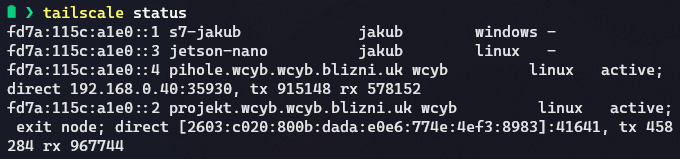
\includegraphics[scale=1]{tailscale-status.png}
    \caption{Status tailscale}
    \label{fig:tailscale_status}
\end{figure}
\begin{samepage}
A także potwierdzić, że nasz adres IP to adres serwera korzystając np. z DuckDuckGo (fig. \ref{fig:ip_check}):
\begin{figure}[H]
    \centering
    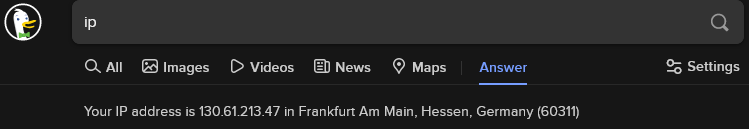
\includegraphics[scale=0.5]{ddg-ip.png}
    \caption{Obecne IP wg. DuckDuckGo}
    \label{fig:ip_check}
\end{figure}
Co jak widać zwraca adres z Frankfurtu, w którym obecnie się nie znajduję.

Patrząc na logi usługi \mintinline{bash}{tailsaled} na serwerze możemy też potwierdzić, że otrzymuje on ruch z klienta (fig. \ref{fig:tailscale-traffic} - klient ma adres 100.64.0.1, a serwer 100.64.0.2)
\begin{figure}[H]
    \centering
    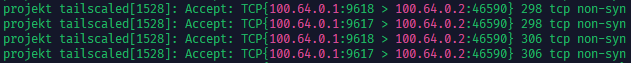
\includegraphics[scale=1]{tailscale-traffic.png}
    \caption{Fragment ruchu na serwerze}
    \label{fig:tailscale-traffic}
\end{figure}
\end{samepage}
\subsection{Wnioski}
Najdłuższą częścią tego projektu (pomijając walkę z Oktą, która tutaj została bardzo delikatnie wspomniana) było pisanie tego raportu, co pokazuje jak prosto jest obecnie skonfiguorwać sensowną sieć wirtualną na własny użytek. Tailscale pozwala nie tylko na wykorzystanie serwera jako krok między komputerem a internetem, ale daje możliwość dostępu do urządzeń gdziekolwiek by nie były praktycznie tak samo łatwo jakby były w sieci lokalnej (a jak nawet widać na fig. \ref{fig:tailscale_status} w przypadku dwóch urządzeń lokalnych połaczenie nawet nie wyjdzie przez internet), bez żadnego pośrednika. Zresztą poza wystawianiem internetu, istnieje możliwość reklamowania sieci lokalnej dając przez jeden "router brzegowy" dostęp do wszystkiego co się w niej znajduje w tailscale (co realizowało by drugą opcję projektu).

Na razie poza ideologiczną chęcią utrzymania kontroli lub specyficznymi wymaganiami nie widzę jednak sensu utrzymywania serwera kontrolnego przy hojnej darmowej ofercie SaaS, więc sam wrócę do tego rozwiązania po projekcie.
\chapter{PiHole}
\label{chap:pihole}
\section{Wybrany sposób realizacji}
Rozwiązanie zostało zrealizowane na osobnym hoście (Nvidia Jetson Nano 2GB) i wykorzystane jako DNS dla sieci Tailscale zrealizowanej w poprzednim zadaniu, w praktyce służąc więc jako DNS dla sieci domowej (a przynajmniej jej części).

Ponieważ urządzenie będzie wykorzystywane też w innych celach, software został zainstalowany w kontenerze dockera z użyciem docker compose.

\section{Instalacja}
\subsection{Instalacja dockera}
Oficjalny obraz od Nvidii na Jetson Nano bazuje na Ubuntu, możemy więc podążyć za oficjalnymi instrukcjami instalacji Dockera na tę dystrybucję (unikając instalowania przez \mintinline{bash}{snap} z powodu wielu problemów jakie ten sposób dystrybucji powoduje w dockerze), które znajdują się pod \url{https://docs.docker.com/engine/install/ubuntu/}
\subsubsection{Instalacja zależności APT}
Do następnych kroków konieczne jest doinstalowanie paczek które pozwolą na dodanie własnego repozytorium APT i używanie go po https
\begin{minted}{bash}
sudo apt-get update
sudo apt-get install \
    ca-certificates \
    curl \
    gnupg \
    lsb-release
\end{minted}
\subsubsection{Dodanie klucza GPG}
Jest to konieczne w celu sprawdzenia podpisów paczek z repozytorium dockera
\begin{minted}{bash}
sudo mkdir -p /etc/apt/keyrings
curl -fsSL https://download.docker.com/linux/ubuntu/gpg \
| sudo gpg --dearmor -o /etc/apt/keyrings/docker.gpg
\end{minted}
\begin{samepage}
    
\subsubsection{Dodanie repozytorium do listy źródeł}
(część tekstu została wydzielona do zmiennych w celu zmieszczenia jej w jednej linii)
\begin{minted}{bash}
ARCH=$(dpkg --print-architecture)
RELEASE=$(lsb_release -cs)
DOCKER_URL=https://download.docker.com/linux/ubuntu
echo \
"deb [arch=$ARCH signed-by=/etc/apt/keyrings/docker.gpg] $DOCKER_URL $RELEASE stable"\
| sudo tee /etc/apt/sources.list.d/docker.list > /dev/null
\end{minted}
\end{samepage}

\subsubsection{Instalacja przez APT}
\begin{minted}{bash}
sudo apt update
sudo apt install docker-ce docker-ce-cli containerd.io docker-compose-plugin
\end{minted}

\subsubsection{Dodanie użytkownika do grupy docker}
\begin{minted}{bash}
    sudo usermod -aG docker $(whoami)
\end{minted}
Po czym należy zakończyć sesję i otworzyć nową (w przypadku połączenia po SSH wystarczy rozłączyć się i połączyć ponownie, pracując bezpośrednio na desktopie należało by się przelogować)

\subsection{Sprawdzenie działania}
Zostało już tylko potwierdzenie, że docker działa przez uruchomienie testowego kontenera który powinien tylko wypisać hello world i zakończy działanie
\begin{minted}{bash}
docker run hello-world
\end{minted}

\subsection{Konfiguracja docker compose}
Ponieważ zamiarem jest wystawienie PiHole w Tailscale potrzebne będą dwie usługi, co najlepiej jest zrealizować przez docker compose.

\subsubsection{Stworzenie folderu na konfigurację}
Do konfiguracji wykorzystałem folder \mintinline{bash}{/srv/pihole}
\begin{minted}{bash}
sudo mkdir -p /srv/pihole
# można też od razu dać swojemu użytkownikowi uprawnienia do folderu
sudo chown $(whoami):$(whoami) /srv/pihole
\end{minted}

\subsubsection{Stworzenie pliku \mintinline{bash}{docker-compose.yml}}
Można w tym momencie użyć preferowanego edytora tekstu
\begin{minted}{bash}
edit /srv/pihole/docker-compose.yml
\end{minted}
\begin{samepage}
Ostateczna konfiguracja obu usług wygląda u mnie następująco:
\begin{minted}{yaml}
version: "3"

services:
  # based on https://github.com/pi-hole/docker-pi-hole/blob/master/examples/docker-compose.yml.example
  pihole:
    container_name: pihole
    image: pihole/pihole:latest
    environment:
      TZ: 'Europe/Warsaw'
      # WEBPASSWORD: 'set a secure password here or it will be random'
      WEBPASSWORD_FILE: '/run/secrets/webpassword' # use a docker secret instead of a static string
      DNSSEC: true
      PIHOLE_DNS_: '1.1.1.1;1.0.0.1;2606:4700:4700::1111;2606:4700:4700::1001'
      WEBTHEME: 'default-auto'
    # Volumes store your data between container upgrades
    volumes:
      - './etc-pihole:/etc/pihole'
      - './etc-dnsmasq.d:/etc/dnsmasq.d'
    restart: unless-stopped
    network_mode: service:tailscale
    secrets:
      - webpassword
    logging: # limit log size
      driver: "json-file"
      options:
        max-size: "100m"
        max-file: "10"
  # adaptation of example command from tailscale docker documentation, also inspired by a few examples online of using it in docker-compose
  tailscale:
    hostname: pihole # this will end up being the name of the tailscale machine
    image: tailscale/tailscale:latest
    volumes:
      - './tailscale:/var/lib' # state files, not necessary but why not
      - '/dev/net/tun:/dev/net/tun' # passing this interface is required
    cap_add:
      # these capabilities are not default, but are required for tailscale to run
      - NET_ADMIN
      - NET_RAW
      # I'm not sure if this is required, but a few docker-compose files with tailscale I've seen did ad dthis
      - SYS_MODULE
    restart: unless-stopped
    command: tailscaled # run the tailscale daemon
    environment:
      TS_EXTRA_ARGS: '--login-server=https://wcyb.blizni.uk' # use a custom login server instead of the tailscale SaaS one
    logging: # limit log size
      driver: "json-file"
      options:
        max-size: "100m"
        max-file: "10"
secrets:
  # use a file from this directory to load the pi-hole admin interface password as a docker secret
  webpassword:
    file: ./webpassword
\end{minted}
\end{samepage}

\subsubsection{Stworzenie pliku z hasłem PiHole}
By uniknąć umieszczenia hasła w pliku konfiguracyjnym wykorzystałem sekret dockera. W przypadku wykorzystania także docker swarm można centralnie zarządzać sekretami, jednak tutaj po prostu oznacza to umieszczenie go w osobnym pliku - \mintinline{bash}{/srv/pihole/webpassword}. Możemy więc wykorzystać dowolny edytor w celu stworzenia tego pliku i wpisania tam naszego hasła
\begin{minted}{bash}
edit /srv/pihole/webpassword
\end{minted}

\subsection{Uruchomienie kontenerów}
By uruchomić wszystko wystarczy wywołać jedną komendę w folderze:
\begin{minted}{bash}
docker compose up -d
\end{minted}
Konfiguracja docker compose oznacza to nawet, że usługi wstaną po restarcie urządzenia (tak długo jak były uruchomione przed restartem).
\subsubsection{Połączenie z tailscale}
Zostało jednak jeszcze połączenie się do ustawionego w \autoref{chap:vpn} serwera headscale. W tym celu należy wykonać komendę w kontenerze tailscale, podobną do tych użytych do dodania serwera i klienta wcześniej (jak i tam można dodać argument \mintinline{bash}{--auth-key} jeśli nie ma się skonfigurowanego dostawcy OIDC):
\begin{minted}{bash}    
docker compose exec tailscale tailscale up \
  --login-server=https://wcyb.blizni.uk \
  --advertise-tags=tag:common
\end{minted}

\section{Konfiguracja Headscale}
W celu użycia PiHole jako serwer DNS w sieci tailscale należy zmodyfikować konfigurację na serwerze (pod \mintinline{bash}{/etc/headscale/config.yaml}) i zmienić konfigurację \mintinline{yaml}{nameservers} na adres IP (IPv4 i/lub IPv6) pihole w sieci tailscale. U mnie będzie to:
\begin{minted}{yaml}
dns_config:
  nameservers:
    - 100.64.0.4
    - fd7a:115c:a1e0::4
\end{minted}
Po zrestartowaniu usługi (\mintinline{bash}{sudo systemctl restart headscale}) urządzenia w sieci powinny już korzystać z PiHole jako DNS (z serwerem Headscale pośredniczącym w celu dodania rekordów dla urządzeń w sieci tailscale), co możemy sprawdzić wyszukując domenę która powinna być zablokowana
\begin{figure}[H]
    \centering
    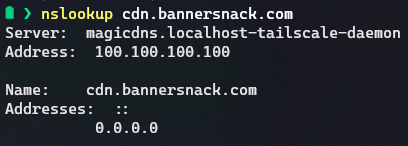
\includegraphics[scale=0.75]{pihole-test.png}
    \caption{Próba znalezienia rekordów dla domeny cdn.bannersnack.com}
    \label{fig:pihole_test}
\end{figure}
\section{Konfiguracja pihole}
Możemy już więc uzyskać dostęp do panelu administracyjnego PiHole przez Tailscale, np. używając stworzonej wewnątrz sieci domeny (u mnie \url{http://pihole.wcyb.wcyb.blizni.uk/}) - powinien nas przywitać ekran logowania (fig. \ref{fig:pihole_login})
\begin{figure}[H]
    \centering
    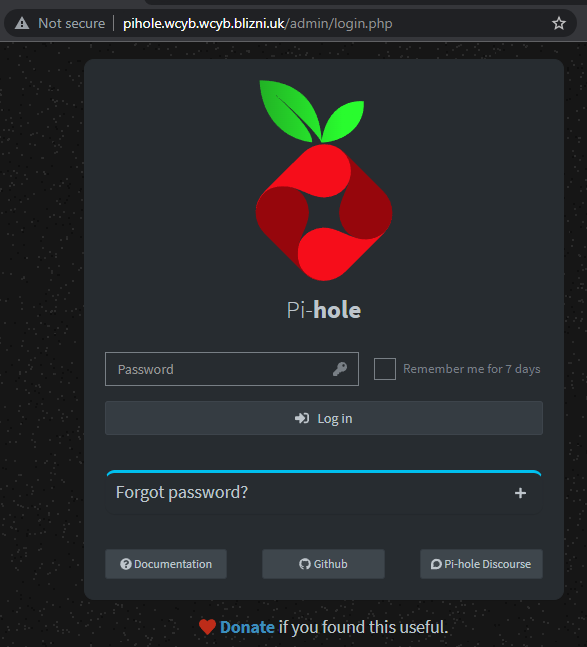
\includegraphics[scale=0.75]{pihole-login.png}
    \caption{Ekran logowania do PiHole}
    \label{fig:pihole_login}
\end{figure}
Po zalogowaniu się stworzonym wcześniej hasłem powinniśmy zobaczyć panel ze statystykami użycia (fig. \ref{fig:pihole_dashboard})
\begin{figure}[H]
    \centering
    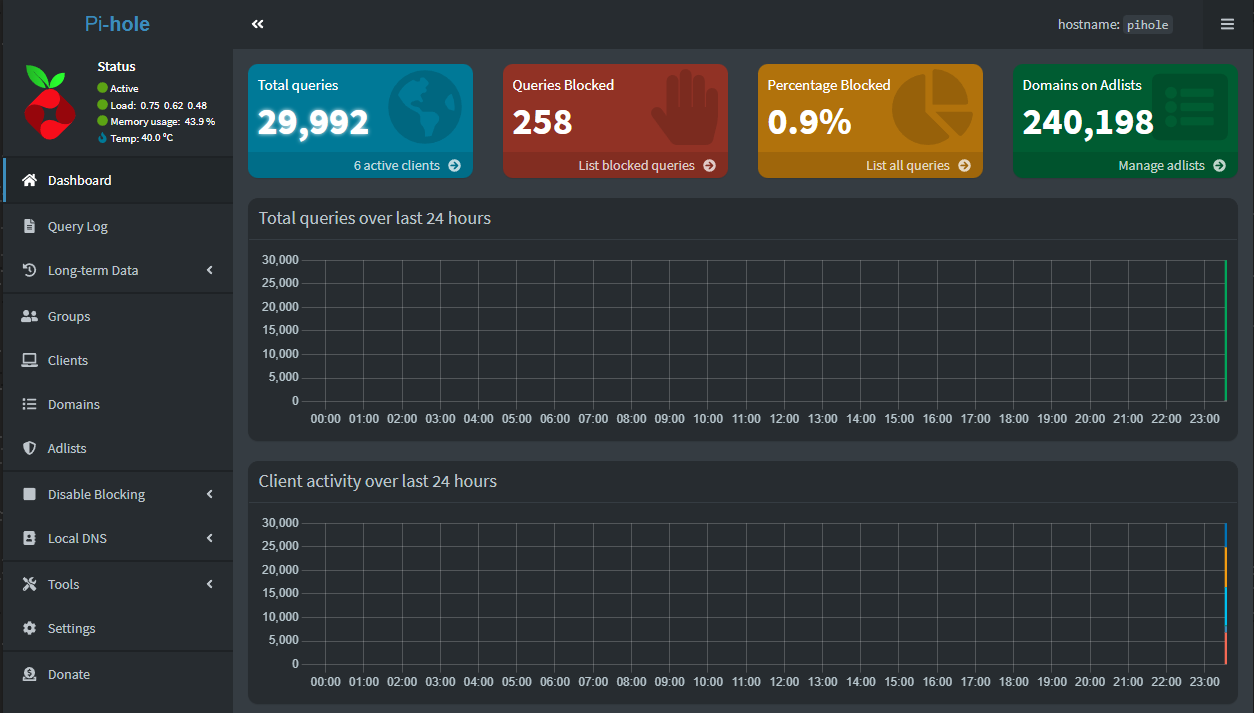
\includegraphics[scale=0.5]{pihole-dashboard.png}
    \caption{Główna strona panelu PiHole}
    \label{fig:pihole_dashboard}
\end{figure}
W panelu jesteśmy w stanie modyfikować część ustawień pihole, manualnie dodawać filtrowane domeny lub wyjątki, dodawać nowe lokalne wpisy DNS, a także aktualizować listy blokowanych domen. Przykładowo dodałem kilka list związanych z bezpieczeństwem (cert.pl, abuse.ch, stopforumspam)
\begin{figure}[H]
    \centering
    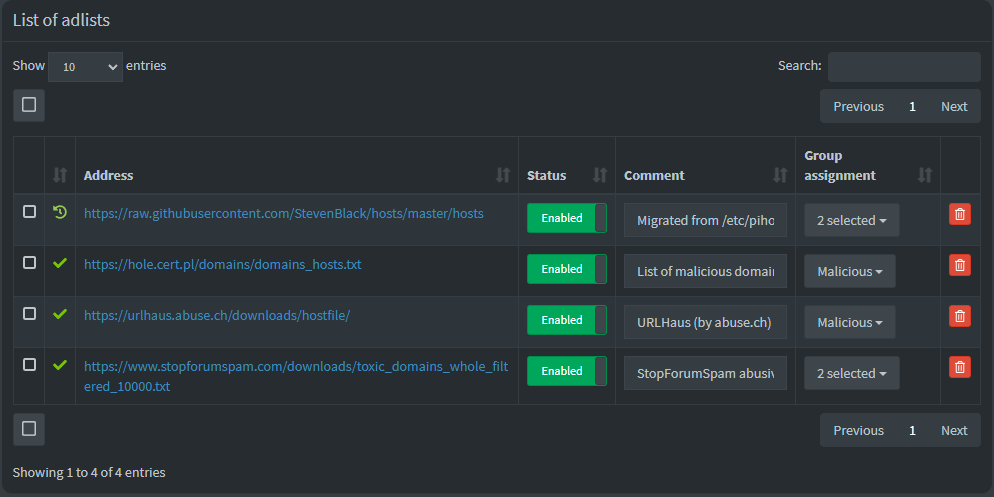
\includegraphics[scale=0.6]{pihole-adlists.png}
    \caption{Listy blokowanych domen w panelu pihole}
    \label{fig:pihole_adlists}
\end{figure}

\section{Podsumowanie}
\subsection{DNS a prywatność}
Operując nawet przez chwilę własny DNS z pełnym logowaniem włączonym nie trudno zauważyć problemu prywatności. Operator jest w stanie prześledzić w zasadzie wszystkie strony do których się łączymy - nawet jeśli nie zna ścieżek na które wchodzimy i nie widzi innych danych żądań, samo to gdzie dany host się łączy stanowi bardzo cenne metadane. A domyślnie wciąż dla większości osób ta masa metadanych trafia do ich operatora internetu, bez żadnego szyfrowania po drodze.

Jednak przez naturę DNS Pi-hole nie do końca rozwiązuje problem jeśli używamy go samemu - kwerendy trafiają do wyższego w hierarchii serwera DNS, nie zmieniając praktycznie nic z ich perspektywy. Dopiero przy większej ilości użytkowników pojawia się zysk w postaci agregacji kwerend (tj. serwer wyżej widzi kwerendy wszystkich jakby pochodziły z jednego urządzenia), ale warto się zastanowić na ile takiej osobie ufamy (chyba, że każdy użytkownik będzie miał dostęp pozwalający sprawdzić, że logowanie domen nie jest włączone w instalacji Pi-hole).

Ale kwerendy DNS nie są jedynym problemem prywatności który Pi-hole potencjalnie adresuje. Drugim, dla większości użytkowników głównym, są reklamy i trackery. Pi-hole wycina je na poziomie DNS, w praktyce po prostu nie pozwalając komputerowi się komunikować ze źródłem reklam i trackerów, tym samym nie dając możliwości nawet ich pobrania. Nie jest to idealne blokowanie - dalej dodatk w przeglądarce może być dobrym pomysłem - ale trudno się kłócić, że jest to poprawa aspektu prywatności w obecnym świecie profilowanych reklam. Jedynym kontrargumentem może być w zasadzie to, że osoby blokujące wszystko też przekazują jakąś informację o sobie (że obchodzi ich prywatność) lub jest to niewystarczające (co niestety można powiedzieć o każdym rozwiązaniu które nie wpływa znacznie negatywnie na doświadczenia korzystania z internetu).

\subsection{DNS a bezpieczeństwo}

Drugą kwestią blisko powiązaną z prywatnością jest bezpieczeństwo. Choć większości osób to nie dotyczy, metadane które wyciekają w naszej historii DNS mogą być jak najbardziej użyteczne dla atakujących z konkretną osobą jako cel. Poznanie np. jakiej poczty email, sieci społecznościowych, usług chmurowych itp. używa pozwala dobrze wycelować choćby atak phishingowy.

Domyślnie większość osób wciąż korzysta z nieszyfrowanych kwerend DNS (choć przeglądarki zaczynają domyślnie włączać DNS over HTTPS), więc nie tylko atak na dostawcę DNS, ale też samo znalezienie się gdzieś w środku trasy wystarczy by poznać o jakie strony dane urządzenie odpytuje.

Konfiguracja Pi-hole, szczególnie w połaczeniu z tailscale, omija to zagrożenie przesyłając cały ruch do Pi-hole przez szyfrowany tunel Wireguard. Bardzo łatwo też ustawić Pi-hole by korzystało z DNS over HTTPS, w praktyce szyfrując cały nasz ruch po drodze.

Dodatkowo samo blokowanie może mieć pozytywny wpływ na bezpieczeństwo - \href{https://cert.pl/posts/2020/03/ostrzezenia_phishing/}{lista ostrzeżeń cert.pl} na przykład zawiera domeny podejrzane o wyłudzanie danych osobowych lub uwierzytelniających, chroniąc przed phishingiem przez po prostu nie pozwolenie się załadować znanym już niebezpiecznym stronom.

\subsection{Alternatywy}
Nie każdy chce jednak hostować własny software. Niestety unikając tego zdajemy się na zaufanie jakiemuś zewnętrznemu dostawy usług. Jeśli jednak to nam pasuje jesteśmy w stanie uzyskać większość zalet Pi-hole korzystając z \href{https://nextdns.io/}{NextDNS}, czyli konfigurowalnego DNSa w formie SaaS.

Jeśli głównie interesuje nas blokowanie reklam to alternatywą (choć nie tylko, bo można korzystać z tego nawet z Pi-hole) jest po prostu adblocker w przeglądarce - np. \href{https://github.com/gorhill/uBlock}{uBlock Origin}.

\end{document}
